\chapter{Meshing}
\label{ref:mesh}
\section{Editing the electrical mesh/layers}
The device structure is split up into layers of different materials.  These can be configured in layer editor which is discussed in section \ref{sec:layereditor}.  Some of these layers will have the layer type 'active'.  An 'active' layer is a layer over which the electrical model will be applied.  The electrical model needs a finite difference mesh to to be setup for it to work.  Usually, this will be take care of automatically, by gpvdm.  However, some users will want fine control over the mesh.  This section describes how to do that. The electrical mesh editor is depicted in figure \ref{fig:emesh}.

The buttons marked 1D, 2D and 3D at the top of the window can be used to toggle the simulation between 1D, 2D and 3D modes.  (Note, if you want to do 2D or 3D simulations you are best off using a default 2D simulation, such as the OFET simulation.  This is because to do 2D/3D simulations, a special newton solver configuration will be needed.) The table on the left hand side is used to configure the mesh.  The sum of the mesh layer thicknesses must exactly match that of the sum of the active layers.  If this is not the case, the model will give an error message.  The columns thickness and mesh points, determine the thickness of the mesh layer and the number of points on the mesh layer, if there is a uniform spacing between mesh points.  The column, 'step multiply' by how much to grow each step.  In this example, the mesh spacing is increased by a factor of 0.1 each step.  The toggle button left/right, defines on which side the mesh layer is generated.  In this example there are two mesh layers, one starting on the left and one starting on the right.  The resulting mesh is plotted in the graph at the bottom of the window.  It can be seen that a non-linear mesh has been generated.

\begin{figure}[H]
\centering
\includegraphics[width=\textwidth]{./images/emesh.png}
\caption{The electrical mesh editor}
\label{fig:emesh}
\end{figure}

\begin{figure}[H]
\centering
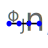
\includegraphics[width=\textwidth]{./images/mesh.png}
\caption{A 1D diagram of the mesh}
\label{fig:emeshdiagram}
\end{figure}

\section{Should I be simulating in 1D, 2D or 3D?}
When deciding if you should perform 1D, 2D or 3D, simulations, consider the dimensionality of your problem.  For example if you consider a solar cell, it is only a few micros thick, and there is rapid variation in the structure, charge densities, mobilities, and doping as a function of depth (y).  However, the structure will not vary very in the lateral (xz) plane.  Therefore, in general  to capture all interesting effects present within a solar cell one only needs a 1D model.  If one now considers OFETs, there is both vertical an lateral current flow, therefore one can not get away with a 1D model any more, as one must simulate both vertical current flow, and current between the source and the drain, thus one needs a 2D simulation.  As the number of dimensions increases, computation speed will decrease, therefore my general advice is to use the minimum number of dimensions possible to solve your problem.

In short try to make your simulation as simple as possible as it will save you time and effort.  Generally the following geometries could be used for various types of devices:

\begin{table}[H]
\begin{center}
\begin{tabular}{ |c|c|c| } 
 \hline
	Device type			& 	Number of dimentions  \\ 
 \hline
	$Solar cells$ 		&	1D \\ 
	$Optical filter$	&	1D\\ 
	$OFET$ 				&	2D\\ 
 \hline
\end{tabular}
\caption{How many dimensions should I use to simulate my device.}
\end{center}
\end{table}

